\section{Discussion}\label{discuss}
%VI.	Discussion
%	a.	\pacora in the Cloud
%	b.	Challenges
%		i.	Outliers/Performance Non-Monotonicity
%			1.	Possible Solutions
%				a.	Heuristics + Feedback
%				b.	Stochastic Models
%		ii.	Variability - can't just average
%			1.	Phases
%			2.	Input Dependent
%			3.	Other � such as network connection
%			4.	Shared Resources
%			5.	Possible Solutions
%				a.	Heuristics + Feedback
%				b.	Stochastic Models
%				c.	Changing Models

There are two main sources of challenges for \pacora's design: performance non-monotonicity and performance variability.  In the following section we describe possible techniques for coping with these challenges.  

The main concern with performance non-monotonicity and variability is that they can possibly effect the accuracy of the response time functions.  However, an interesting result we have found while evaluating \pacora is that model accuracy has less impact on the quality of resource allocation decisions than anticipated.  When experimenting with possible models for the RTF functions, we found that while some models were always a little too inaccurate and did degrade the performance of the resource allocation decisions, once a model crossed a certain threshold of accuracy then better models provided insignificant improvement in resource allocation decisions~\cite{pacora_tr}. Figure~\ref{accuracy_quality} shows the effect of model accuracy on the quality of the resource allocation decisions made using RTF model in Equation~\ref{rtf_eq}.  Although there is a slight correlation between model accuracy and decision quality, many decisions with inaccurate models still result in near optimal allocations.
\begin{figure}[!t]
	\begin{center}	
%		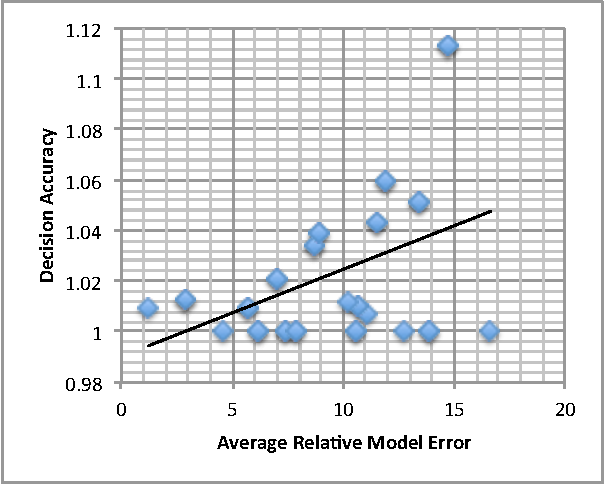
\includegraphics[width=0.9\textwidth]{cluster_decision_accuracy.pdf}
		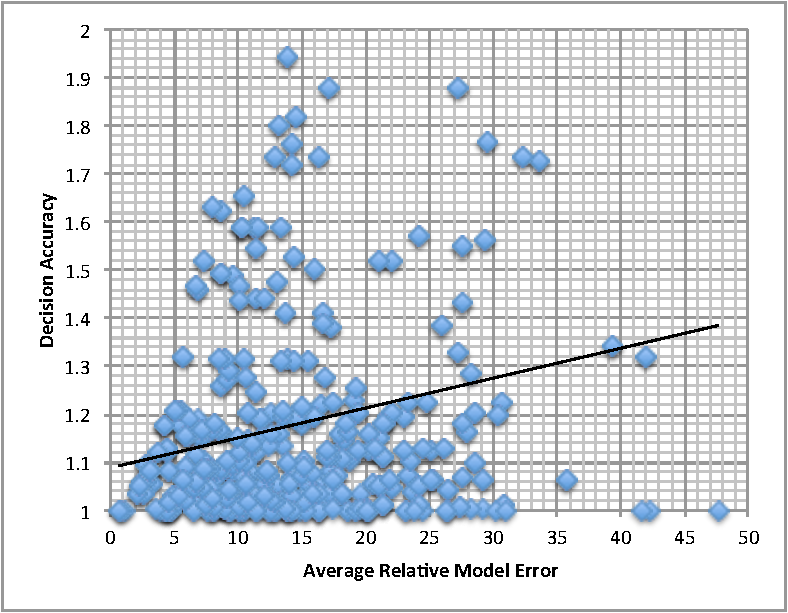
\includegraphics[width=0.9\columnwidth]{parsec_decision_accuracy.pdf}
		\caption{Effect of Model Accuracy on Decision Quality}
		\label{accuracy_quality}
	\end{center}
\end{figure}

\subsection*{Outliers and Performance Non-Monotonicity}


Discuss Heuristics + Feedback
\subsection*{Variability}
Discuss phases, input dependence, other variability (such as network connection), shared resources

Possible solutions include Heuristics + Feedback, Stochastic Models, Changing Models

%Program phase detection has targeted hardware or software reconfiguration. The overview~\cite{dhodapkar-micro03} evaluates three measurement-based predictors, and while performance variation is not one of the three, the authors note that small performance variation is an indicator of correct phase identification.  A similar conclusion is reached in~\cite{sherwood-sigarch03}.

% don't forget cpu frequency

Obviously there may always be some shared resources; however, we have found a trend towards minimizing interference in emerging chip-designs as efficiency and predictability begin to trump utilization as primary concerns.




